% =====================================================================
% AttentionSeekers: end-submission report.
% Each file in sections/ carries a FLOW comment before every paragraph:
%   STEP | CHARACTER (the paragraph's grammatical subject) | HAND-OFF
% plus SOURCE notes for every number. Rewrite prose freely, but keep what
% the FLOW says the paragraph must do.
% Orange \pending{} text marks content that waits on the end-submission
% runs. Search for "\pending" before submitting.
%
% Template: ACL (acl.sty and acl_natbib.bst from github.com/acl-org/
% acl-style-files, downloaded 2026-10-31). Option "preprint" shows authors
% and page numbers; use "review" for an anonymous submission or "final" for
% camera-ready. acl.sty itself loads geometry, natbib, hyperref and the
% bibliography style, so do not load them again here.
% =====================================================================
\documentclass[11pt]{article}
\usepackage[preprint]{acl}
\usepackage{times}
\usepackage{latexsym}
\usepackage[T1]{fontenc}
\usepackage[utf8]{inputenc}
\usepackage{microtype}
\usepackage{inconsolata}
\usepackage{graphicx}
\usepackage{amsmath,amssymb}
\usepackage{booktabs}
\usepackage{tabularx}
\usepackage{xcolor}

% Pending content (remove every use before submitting).
\newcommand{\pending}[1]{\textcolor{orange!85!black}{[PENDING: #1]}}
% Notation used across sections.
\newcommand{\smh}{style heads}

% TITLE: the proposal title ("Causal Disentanglement of User-Induced and
% Assigned Persona in Language Models") claims a disentanglement we have not
% shown. Options: (a) "Do Language Models Mirror Users Through Their Persona
% Heads?"; (b) "User Style and Assigned Persona in Language Models: Shared
% Heads, Separate Paths?" (only if the removal results support it); (c) keep
% the proposal title. Decide after the removal results.
\title{Do Language Models Mirror Users Through the Heads That Carry Their Persona?}
\author{Ronit Jalihal \And Bhavya Ahuja \AND Eshaan Sharma \And Krishak Aneja}

\begin{document}
\maketitle

% =====================================================================
% ABSTRACT. ~150-180 words. No model, dataset or metric names; at most
% one number; no inferential terms. Each sentence's subject entered as an
% object in the sentence before (characters: assistants -> the two
% sources -> we -> these inputs -> the model -> the heads -> these heads).
% =====================================================================
\begin{abstract}
% FLOW S1-S2: stakes, then why the question matters | CHARACTER: assistants,
% then the two sources | HAND-OFF: matched inputs
Chat assistants take on personality from two sources: the persona their system prompt assigns, and the style in which the user writes. Whether the two reach the model through the same internal machinery decides whether one can be controlled without disturbing the other.
% FLOW S3-S4: what we built and measured | CHARACTER: we | HAND-OFF: the model
We build matched inputs in which a personality moves between the system prompt and the user's message while the request and a fixed assistant reply stay the same. A judge that never sees the user's message scores the replies the model generates freely.
% FLOW S5-S6: findings | CHARACTER: the model -> the style heads
The model mirrors a user's enthusiasm but not their reserve. Attention heads previously shown to carry an assistant's persona rank first in their layer whether the system prompt changes its personality or only its wording. The user moves them only weakly and in a different direction, and switching them off leaves mirroring intact.
% FLOW S7: the removal result | SOURCE: ada/report/metrics.json
Removing the user's style direction from the residual stream at their layer reduces mirroring by roughly 30\%, with a wide interval. Removing the user's direction from these heads, or from any other head group we tested, leaves mirroring unchanged.
% FLOW S8: what follows, scoped to a single turn
In a single turn, these heads register the user's style but are not needed for mirroring.
\end{abstract}

% =====================================================================
% INTRODUCTION. Expands the abstract in its order: S1-S2 -> P1-P2, S3 -> P3,
% S4 -> P4, S5-S7 -> P5, contributions -> P6. Citations only in P1-P2.
% No symbols or equations. Results stated as adjectives, not numbers.
% =====================================================================
\section{Introduction}
\label{sec:intro}

% FLOW P1: stakes | CHARACTER: assistants | HAND-OFF: ends on "two sources"
% NOTE: Lu et al.'s drift is away from the DEFAULT assistant persona, not
% from a persona assigned by a system prompt (plan_agent.md 2.10). Keep it.
Chat assistants are usually given a persona. A system prompt describes how the assistant should sound, and the persona it describes corresponds to directions inside the model that can be measured and steered \citep{chen2025persona}. In conversation, assistants also move towards the personality of the user they are talking to, a behaviour earlier work calls personality mirroring \citep{sprejer2026white}. Over long conversations they drift away from their default assistant persona \citep{lu2026assistant}. An assistant's personality therefore has two sources: the system prompt it is given and the way the user writes.

% FLOW P2: the gap; the only paragraph where criticism has its own clause |
% CHARACTER: the two sources -> the evidence for each | HAND-OFF: ends on
% "a test that holds everything fixed except where the personality comes from"
The two sources are not equally well understood. The assigned persona has been traced to a sparse set of attention heads that write an assistant's style \citep{izawa2026steering}. The user's side is known only from model-wide correlations: activations move along trait components after a user interacts with the model, and \citet{sprejer2026white} leave open whether that movement reflects the model's own persona or its representation of the user's style. Two obstacles stand in the way of an answer. In real conversations the two sources co-occur and differ in content, so their effects cannot be separated, and a shift in activations cannot by itself distinguish perceiving the user's style from adopting it. The answer matters for control, because if both sources share machinery, suppressing mirroring would also damage the persona the assistant was given. Separating them requires a test that holds everything fixed except where the personality comes from.

% FLOW P3: what we offer; the design choice explained in one sentence |
% CHARACTER: we -> the inputs | HAND-OFF: ends on "these inputs"
We build such a test. Within a request, our inputs differ only in personality: where it sits, in the system prompt or in the user's message, and which end of a trait it expresses (Figure~\ref{fig:design}). The request and the assistant's reply are identical across all inputs built from it. We study two Big Five traits, extraversion and agreeableness, at their high and low ends, across requests from four everyday domains, and we check every user rewrite to confirm that it asks for the same thing as the original. All experiments use single exchanges with one open-weight model.

% FIGURE 1 does argumentative work here: one request, three placements of
% the personality, one shared reply. Real rows from the dataset (code_01).
% Full width (figure*): it floats to the top of the next page.
\begin{figure*}[t]
\centering
\small
\begin{tabularx}{\textwidth}{@{}lX@{}}
\toprule
\textbf{Neutral} & \textit{System:} You are a helpful assistant.\\
 & \textit{User:} How do I reverse a singly linked list in Python?\\
\midrule
\textbf{User rewrite (E+)} & \textit{System:} You are a helpful assistant.\\
 & \textit{User:} Hey! I'm really curious about reversing a singly linked list in Python. How do I do that?\\
\midrule
\textbf{System twin (E+)} & \textit{System:} You are an extraverted assistant. Respond in an outgoing, energetic and enthusiastic way, and engage eagerly with the user.\\
 & \textit{User:} How do I reverse a singly linked list in Python?\\
\midrule
\textbf{Shared reply} & Reversing a singly linked list in Python can be done using various methods. One common approach is to use a loop to iterate through the list and reverse the pointers.~\ldots\\
\bottomrule
\end{tabularx}
\caption{One request in three forms. The high-extraversion personality sits either in the user's message or in the system prompt, while the request and the assistant's reply stay the same. Low-extraversion versions are built the same way.}
\label{fig:design}
\end{figure*}

% FLOW P4: how we use the inputs + how we know it works | CHARACTER: these
% inputs -> the measurements | HAND-OFF: ends on mirroring / the tests
% No machinery names here (no "permutation", "lambda", "cross-fitting").
These inputs let us compare which attention heads respond to each source, including the heads that earlier work found to write an assistant's style, which we call the style heads. They also let us measure mirroring directly: the model answers each user message freely, and a judge that never sees the user's message scores the personality of the reply. Finally, we test causally, by switching the style heads off and by removing only the user-style direction from their output, from their whole layer and from the residual stream. Our extraction code matches the original implementation on the inputs we tested. Each head-level edit is compared with random heads or a random direction, and each direction is applied only to requests it was not estimated on.

% FLOW P5: findings as adjectives (one number: ~30%) | CHARACTER: the model
% -> the style heads -> the removal | HAND-OFF: to the contributions
% SETTLED: the wording-only control also puts the style heads on top, so
% they are described as the heads most sensitive to the system prompt, with
% head 2 alone responding to personality beyond rewording.
The model mirrors a user's enthusiasm but not their reserve. Its replies become clearly more extraverted when the user writes in a sociable or energetic way, while replies to reserved users barely change, and neither absolute nor pairwise judging detects any mirroring of agreeableness. The style heads turn out to rank first in their layer whether the system prompt changes its personality or only its wording, and only one of them responds to personality well beyond a rewording. The user's style reaches the same heads, but weakly and in a different direction from the system prompt, and switching the heads off, or removing only the user's direction from them, leaves mirroring intact. Removing the user's direction from the residual stream of their layer reduces mirroring by roughly 30\%, with a wide interval, while the assigned persona keeps almost all of its effect.

% FLOW P6: contributions, prose, ordinals, no numbers, no overlap; the
% dataset first | CHARACTER: each contribution names its object
We make three contributions. First, a dataset that isolates where a personality comes from, with a quality-check protocol that pairs a checklist judge with a blind comparison against the original message. Second, a comparison of the two sources on the same attention heads, with causal tests against random controls. Third, evidence that single-turn mirroring is selective: it follows a user's enthusiasm but not their reserve, and depends on which facet of the trait the user expresses.

% =====================================================================
% RELATED WORK. Four paragraphs, from the phenomenon to the mechanism,
% ending on the work we build on directly. Describe prior work in its own
% terms; criticism only in subordinate clauses. TRAP: never say a component
% "carries" or "drives" a behaviour unless the cited work intervened.
% Citation fixes still open: Lu et al. (title/authors), Izawa et al.
% (authors), Sprejer et al. (authors). See references.bib.
% =====================================================================
\section{Related Work}
\label{sec:related}

% FLOW RW1: viability, personality is measurable in text | CHARACTER:
% personality -> language models | HAND-OFF: ends on models expressing
% personas that prompts can set
% Trimmed 2026-10-31 for the 8-page limit: four paragraphs -> three.
% FLOW RW1: personality and persona directions | HAND-OFF: where is it written
\paragraph{Personality and persona.}
The Big Five describes personality along five traits, each divided into facets \citep{soto2017next}, and personality leaves measurable traces in writing \citep{pennebaker1999linguistic, mairesse2007using}. Language models express personas that a prompt can set: traits such as sycophancy correspond to directions in a model's activations that can monitor and steer its persona \citep{chen2025persona}, and steering vectors more generally shift what a model generates \citep{subramani2022extracting}. These methods act on the residual stream as a whole, which leaves open where in the network a persona is written.

% FLOW RW2: mirroring and drift | HAND-OFF: fixed positions, fixed content
\paragraph{Mirroring and drift.}
Over long conversations, assistants depart from their default persona, and clamping activations along a single assistant direction reduces the departure \citep{lu2026assistant}. Assistants also shift towards the user's personality: their activations move along trait components after users interact with them, and \citet{sprejer2026white} leave open whether this reflects the model's own persona or its representation of the user's style. Inside the model the boundary between user and assistant roles is weak, and style can dominate role markers \citep{ye2026prompt}, so probes trained across positions can confuse whose style they detect. We therefore read activations at fixed positions and hold content fixed.

% FLOW RW3: persona in components | HAND-OFF: the question our dataset answers
\paragraph{Persona in specific components.}
Activation patching has located persona-driven reasoning in specific components of a model \citep{poonia2025dissecting}. Most directly, \citet{izawa2026steering} find that a sparse set of attention heads, which they call style modulation heads, writes an assistant's style, and validate them with system prompts and steering. Their personas are assigned through the system prompt and are not Big Five traits, and they do not test a style that arrives through the user's message.

% =====================================================================
% DATASET. Opens on the one property the dataset is built around, then
% follows the order of construction. Every number checked against
% Data_Creation/data on 2026-10-31. Re-check if the data are regenerated.
% =====================================================================
\section{Dataset}
\label{sec:dataset}

% FLOW D0: the design property, in one sentence, not defended | CHARACTER:
% the dataset | HAND-OFF: to the traits and requests that fix the content
No dataset we know of holds a conversation's content fixed while moving its personality between the system prompt and the user. We therefore built one around a single property: within a request, any two inputs differ only in personality, never in what the user asks or in the assistant's reply.

\subsection{Traits and requests}
% FLOW D1: traits, then requests | CHARACTER: the traits -> the requests |
% HAND-OFF: ends on the neutral message, whose reply D2 introduces
% SOURCE: scenarios.jsonl (20 requests, 5 per domain); prompts.py
We study extraversion and agreeableness, each with a high and a low pole. We define each pole through the three BFI-2 facets of its trait \citep{soto2017next}, together with marker adjectives \citep{saucier1994mini} and the linguistic cues of each trait \citep{pennebaker1999linguistic, mairesse2007using}. We use the BFI-2 rather than the NEO-PI-R because the NEO-PI-R places warmth under extraversion, which would blur the two traits we want to keep apart. The requests come from four everyday domains, coding, explanation, emotional advice and brainstorming, with five requests each. The emotional-advice requests are adapted from the request categories in \citet{li2025human}. Each request has a one-line intent and a neutral user message without personality markers, such as ``How do I reverse a singly linked list in Python?''. Concrete details in the neutral message, such as the programming language or the user's nationality, pin down what is asked, so that rewrites cannot drift in content.

\subsection{Fixed replies}
% FLOW D2: the fixed reply | CHARACTER: the reply | HAND-OFF: ends on the
% reply being shared by every input of its request
% SOURCE: qc/forced_responses/raw_long.jsonl (min 90, median 620, max 1024,
% one unfinished). The causal-attention equivalence is in Method 4.1.
Every input built from a request shares one assistant reply. The studied model wrote these replies itself, by greedy decoding from the neutral system prompt ``You are a helpful assistant.'' and the neutral message. We store each reply in full, capped at 1,024 tokens. The replies run from 90 to 1,024 tokens, with a median of 620, and the one reply that reached the cap was cut at its last complete sentence. Section~\ref{sec:readouts} explains why storing the full reply costs nothing when activations are read over a shorter window.

\subsection{User rewrites}
% FLOW D3: the rewrites and how they are generated | CHARACTER: the
% rewrites | HAND-OFF: ends on the prompt's prohibitions -> the check (D4)
% SOURCE: user_variants.jsonl (240 rows; qc.facet = 20 per k per trait);
% prompts.py. Rewrite index = facet is flagged in Limitations.
A rewrite restates the neutral message in one pole of one trait and asks for exactly the same thing. For each request, trait and pole we wrote three rewrites, giving $20 \times 2 \times 2 \times 3 = 240$. Each of the three leads with a different facet of the trait: sociability, assertiveness or energy for extraversion, and compassion, respectfulness or trust for agreeableness (Table~\ref{tab:facets} in Appendix~\ref{app:tables}). The low pole uses the low end of the same facet, so the $k$-th high and low rewrites of a request form a facet-matched pair. A generator model, DeepSeek-V4.1-Flash, wrote the three rewrites of each cell in one call, from the pole's definition and cues, the facet assigned to each rewrite and four out-of-domain examples. Its instructions forbid adding facts, adding constraints on the answer such as ``just give me the code'', and keeping the original wording with a styled sentence appended.


% FLOW D4: the quality check and its outcome (details moved to Appendix D)
% | CHARACTER: each rewrite -> the outcome | HAND-OFF: ends on length per
% pole | SOURCE: run_config.json (generator deepseek-flash, judge
% gpt-6-luna, max_attempts 5); qc.attempts = 143/82/10/5; Qwen token means
% E 36.0 vs 24.6, A 39.7 vs 29.2. Human audit: 0 of 24 done.
Each rewrite then had to pass three checks (Appendix~\ref{app:qc}). Automatic checks bounded its length and rejected copies of the neutral message. A judge model, GPT-6 Luna, answered nine yes/no questions on content, style boundaries and realism (Appendix~\ref{app:checklist}), since decomposed questions are more reliable for model judges than a single score \citep{cook2024ticking, qin2024infobench, lee2024checkeval}. Finally, the judge saw the neutral message and the rewrite side by side, in both orders to cancel position bias \citep{zheng2023judging}, and picked the writer who sounds more extraverted or more agreeable. A high-pole rewrite had to win both times, and a low-pole rewrite had to lose both times. Failed rewrites were regenerated with the judge's reasons as feedback. All 240 rewrites passed, 143 of them on the first attempt and none after the fourth. High-pole rewrites are longer than low-pole ones, at 36.0 against 24.6 tokens for extraversion and 39.7 against 29.2 for agreeableness, and we record each rewrite's length. \pending{human audit of a random 10\% sample (24 rewrites): report agreement with the judge, or delete this sentence.}

\subsection{System-prompt twins}
% FLOW D5: the twins (behavioural check moved to Appendix C) | CHARACTER:
% the twins | HAND-OFF: to the crossed set
% SOURCE: sys_prompts.json (20 prompts; clause on the 10 A prompts);
% persona_check v1/v2; DECISIONS.md D8.
A system twin keeps the neutral message and the fixed reply and moves the personality into the system prompt. We wrote five system prompts per trait and pole in the format of \citet{chen2025persona} and \citet{izawa2026steering}, ``You are a [X] assistant. [instruction]'', writing each high-pole prompt in parallel with its low-pole counterpart (Appendix~\ref{app:sysprompts}). This gives $20 \times 2 \times 2 \times 5 = 400$ twins, plus 20 neutral rows that pair the neutral message with the neutral system prompt. A behavioural check showed that the low-agreeableness prompts made the model withhold help, so the agreeableness prompts also ask it to keep helping (Appendix~\ref{app:syscheck}).

\subsection{Crossed set}
% FLOW D6: the crossed set + summary table | CHARACTER: the crossed set |
% HAND-OFF: to Method (how activations are read on these inputs)
% SOURCE: factorial.jsonl (720 rows; sys k paired with user k: verified)
The crossed set pairs every system-prompt condition (high, low, none) with high and low user rewrites, matching system prompt $k$ with rewrite $k$. It has 360 rows per trait. Appendix~\ref{app:tables} summarises all four sets (Table~\ref{tab:sets}).



% =====================================================================
% METHOD. Five subsections in the order Results uses them. Machinery is
% named here. Vocabulary: "reference run" (never "baseline"); lambda = 1
% "removes", lambda = 2 "steers".
%
% TWO REGIMES; never put numbers from both in one sentence or table:
%   Regime 1 (earlier runs): bf16, RTX 3090, sampled generation.
%   Regime 2 (removal runs): fp16 sharded over two 11 GB GPUs (model not
%            recorded in the run files; do not name it), greedy decoding,
%            150 new tokens (arm.json: temperature 0.0, max_new_tokens 150).
% VERIFIED against code at commit fc1dbd3: Workstream_2 chat.py, extract.py,
% heads.py, configs/qwen.json, configs/qwen_ada.json (dtype float16);
% Workstream_3 generate.py (projection_hook), residual.py
% (layer_output_hook), directions.py, project.py, pairwise.py,
% judge.py, rubrics.py, mirroring.py, factorial.py, ablate.py, compare.py,
% diagnostic.py; and every ws3_results/ada/*/arms/*/arm.json.
% =====================================================================
\section{Method}
\label{sec:method}

\subsection{Model and activation readouts}
\label{sec:readouts}
% FLOW M1a: the model and the style heads | CHARACTER: the model -> the
% style heads | HAND-OFF: ends on the heads' outputs, which M1b reads
% SOURCE: configs/qwen.json
We study Qwen2.5-7B-Instruct \citep{qwen2025technical} (revision \texttt{a09a354}), which has 28 layers of 28 query heads, each of dimension 128. \citet{izawa2026steering} report three style modulation heads for this model, heads 2, 4 and 27 of layer 19 in zero-indexed numbering; their paper numbers them heads 3, 5 and 28 of layer 20. We call them the style heads.

% FLOW M1b: the three readouts and why the full reply is stored | CHARACTER:
% each head's output -> the readouts | HAND-OFF: to the implementation check
% SOURCE: chat.py encode(); extract.py capture_encoded() (prompt-only pass
% for first/user); qwen.json response_tokens = 150
For head $i$ of layer $\ell$ we record its slice $z_{\ell,i} \in \mathbb{R}^{128}$ of the input to the layer's attention output projection $W^O_\ell$. We read it at three positions. The \emph{first} readout is the last token of the prompt, which predicts the first reply token; we take it from a forward pass over the prompt alone, so the reply cannot affect it. The \emph{response} readout is the mean over the first 150 tokens of the fixed reply, fed to the model as if it had written it, which is the readout of \citet{izawa2026steering}. The \emph{user} readout is the mean over the tokens of the user's message. We tokenize the prompt and the reply separately and join their token IDs, so no token spans the boundary. Attention is causal, so averaging the first 150 tokens of the full reply gives exactly the activations a 150-token reply would give, which is why the dataset stores full replies.

% FLOW M1c: the implementation check, scoped precisely | CHARACTER: our
% code | HAND-OFF: to localization (M2)
% SOURCE: full_qwen_verification_summary.json (rows brainstorm_01|S|E|+|k0
% and brainstorm_01|S|E|-|k0; max score error 1.335e-5; Spearman 1.0)
On one request's high- and low-extraversion system twins, our code and the original implementation of \citet{izawa2026steering} give identical activations and head scores within $1.3 \times 10^{-5}$. This confirms that we compute the same quantities but does not reproduce their experiments.

\subsection{Locating heads that respond to a personality}
\label{sec:localize}
% FLOW M2a: the contrast | CHARACTER: a pair -> the contrast | HAND-OFF:
% ends on delta, which the score in M2b uses
% SOURCE: heads.py paired_scenario_differences(), matched_pairs()
For one trait and one source of personality, a pair is two inputs that differ only in pole. Assigned contrasts pair system twins, 100 pairs per trait; user contrasts pair user rewrites, 60 pairs per trait. For each request $b$ we average the pair differences $z_+ - z_-$ over its paraphrases to obtain $d_b$, and average over requests to obtain the contrast $\delta = \frac{1}{B}\sum_b d_b$.

% FLOW M2b: the head score and the test | CHARACTER: the score -> the test
% | HAND-OFF: ends on "ranks and effect sizes", which M2c compares
% SOURCE: heads.py head_contributions(), sign_flip_pvalues() (19,999 flips,
% one-sided), bh_qvalues()
The contribution score of head $i$ in layer $\ell$ follows \citet{izawa2026steering}:
\begin{equation}
s_{\ell,i} = \Big\langle W^O_{\ell,i}\,\delta_{\ell,i},\ \sum_{j} W^O_{\ell,j}\,\delta_{\ell,j} \Big\rangle ,
\end{equation}
the projection of the head's write onto the layer's total write. The scores of a layer sum to the squared norm of the layer's total write, so they decompose that layer, and we rank heads within their layer. For significance we flip the signs of whole requests' differences $d_b$ (19,999 flips in the main runs and 999 in the half-precision re-run, one-sided) and correct across all 784 heads with the Benjamini--Hochberg procedure \citep{benjamini1995controlling}. Requests, not paraphrases, are the unit of resampling, because paraphrases of one request are not independent.

% FLOW M2c: comparing the two sources + the wording-only control |
% CHARACTER: the comparisons | HAND-OFF: to mirroring (M3)
% SOURCE: cli.py cmd_compare (Spearman over 784 heads); ws3/compare.py
% (1,000 random triples); ws3/diagnostic.py (same-pole k0 vs k1, saves
% smh_ranks_in_layer; ada/jobA/analysis/same-pole/metrics.json, 999 flips).
% The fp16 re-run (ada/jobA/analysis) reproduces the bf16 ranks exactly.
We compare the two sources by the Spearman correlation of their head scores over all 784 heads and by the ranks of the style heads under each source. We also compute the cosine between the assigned and user contrasts restricted to the style heads, a 384-dimensional vector, and compare it with the same cosine for 1,000 random three-head groups in layer 19. As a control on the ranking itself, a wording-only contrast pairs two different system prompts of the same pole ($k=0$ against $k=1$). It changes how the system prompt is worded without changing the trait, so heads that rank highly under it respond to wording rather than to personality.

\subsection{Measuring mirroring}
\label{sec:mirroring}
% FLOW M3a: generation, two regimes | CHARACTER: the model's free replies |
% HAND-OFF: ends on the replies the judge scores
% SOURCE: Workstream_3/configs/ws3.json (temperature 1.0, 300 tokens,
% 2 samples per rewrite, 3 per neutral message = 540 replies); removal runs:
% project.py + arm.json (greedy, 150 tokens, 120 mirroring + 80 2x2).
The model answers each user rewrite under the neutral system prompt. For the behavioural comparison we sampled at temperature 1.0, with replies of up to 300 tokens, two replies per rewrite and three per neutral message, 540 replies in total. For the removal experiments (Section~\ref{sec:removal}) we decode greedily with replies of up to 150 tokens, one reply per rewrite, so that a run differs from its reference run only through the intervention.

% FLOW M3b: the judge and the mirroring effect | CHARACTER: the judge -> the
% effect | HAND-OFF: to the pairwise judge for agreeableness (M3c)
% SOURCE: judge.py (GPT-4.1-mini, top-20 logprobs, min integer mass 0.25);
% rubrics.py (no user text; refuses records containing the user message);
% mirroring.py (Wilcoxon, d_z, 5,000 request resamples)
Following \citet{izawa2026steering}, a judge, GPT-4.1-mini, scores each reply from 0 to 100 for extraversion, agreeableness, coherence and refusal, as the probability-weighted mean over its top 20 integer tokens. The judge sees the reply and the request's neutral intent but never the user's message, so it cannot score the user's style instead of the model's. For trait $t$, the mirroring effect is
\begin{equation}
M_t = \frac{1}{B}\sum_{b=1}^{B}\left(\bar y_{b,+} - \bar y_{b,-}\right),
\end{equation}
where $\bar y_{b,\pm}$ is the mean judged score of trait $t$ over request $b$'s replies to its high- or low-pole rewrites. We test $M_t$ with a Wilcoxon signed-rank test over the 20 requests and report Cohen's $d_z$ with a 95\% confidence interval from 5,000 request resamples.

% FLOW M3c: pairwise judging for agreeableness | CHARACTER: the pairwise
% judge | HAND-OFF: to the regression (M4)
% SOURCE: ws3/pairwise.py (both orders, probability-weighted choice,
% p_high averaged over orders; sees the intent and two replies only).
Absolute agreeableness scores sit near the top of the scale for every pole (Section~\ref{sec:results}), which leaves no room to detect a shift. We therefore also judge agreeableness pairwise, and extraversion as a check, on the greedy replies of the reference run (Section~\ref{sec:removal}). The judge sees the replies to a request's high- and low-pole rewrites, again without either user message, and picks the one with more of the trait, once in each order. We report the probability that the reply to the high-pole user is chosen, averaged over both orders, so that 0.5 means no mirroring.

\subsection{Separating the two sources in the activations}
\label{sec:regression}
% FLOW M4: the crossed-set regression (details moved to Appendix E) |
% CHARACTER: a head group's activations | HAND-OFF: to the causal tests
% SOURCE: factorial.py (CODES, BLOCKS, center_within, 1,000 bootstraps and
% shuffles)
On the crossed set, a regression splits a three-head group's activations into what the system prompt explains and what the user's style explains. We regress the group's 384-dimensional activations, centered within each request, on orthogonal codes for the system prompt's pole and presence, the user's pole and their interactions, and report the variance each block explains and the cosine between the system-prompt and user coefficients (Appendix~\ref{app:regression}). We fit it for the style heads, the three heads of layer 19 with the largest mean activation norm on neutral inputs (a control for head size) and five random triples, for extraversion only.

\subsection{Causal tests}
\label{sec:causal}
% FLOW M5a: zeroing | CHARACTER: the style heads | HAND-OFF: ends on
% "needed", which M5b narrows to "what they carry"
% SOURCE: generate.py zero_head_hook (every position); ablate.py
Zeroing tests whether the style heads are needed for mirroring. We set their slices of the output-projection input to zero at every position during generation, repeat the mirroring measurement, and compare with zeroing random three-head groups from the same layer.

\label{sec:removal}
% FLOW M5b: direction removal | CHARACTER: the user-style direction -> the
% hook -> the arms | HAND-OFF: to Results
% VERIFIED (code + arm.json): hooks act at every position (prompt and
%   generated tokens; generate.py projection_hook, residual.py
%   layer_output_hook); u = unit mean user contrast on the resp readout of
%   the training requests; mu_0 = mean of neutral rows of the training
%   requests; 4 folds by request, domains spread across folds (directions.py
%   assign_folds); random triple = heads 14, 17, 21 (excludes 2, 4, 27);
%   top-10 heads by raw user score per fold (fold 0: L19 h2, L26 h10/12,
%   L27 h7-13); random direction = random unit vector in the 3,584-dim
%   layer-19 head space; greedy, 150 tokens; 120 mirroring + 80 2x2 replies
%   per arm. lambda = 0 identity is checked by ws3/ada_smoke.py (the smoke
%   run log is not in the repository).
Removing a direction is narrower than zeroing: during generation, at every position, a hook replaces a group's output $z_G$ by
\begin{equation}
z_G \leftarrow z_G - \lambda\, u u^{\top} (z_G - \mu_0),
\end{equation}
where $u$ is the unit user contrast of group $G$ on the response readout and $\mu_0$ is the group's mean on neutral inputs, both computed on training requests only. With $\lambda = 1$ the hook removes the user-style component and leaves the rest of the output unchanged; with $\lambda = 2$ it reflects the component, which is intended to steer the output towards the opposite style. Each group uses its own direction, and we apply every direction only to requests it was not estimated on: the 20 requests are split into four folds, each held-out request is generated with a direction fit on the other 15, and the top user-style heads are chosen within each fold. We remove the direction from the style heads, from a random triple without them, from all 28 heads of layer 19, from the ten most user-responsive heads in any layer and from the residual stream after layer 19, and remove a random direction from layer 19's heads as a control. We also reflect it in the style heads and in all heads of layer 19 (Appendix~\ref{app:arms}). Each arm is compared with an unhooked reference run from the same job on the reduction in mirroring, $1 - M_{\text{arm}}/M_{\text{ref}}$, with a paired request-bootstrap interval. It is also compared on persona preservation: on the corner of the crossed set that pairs a high or low system prompt with a high or low rewrite ($k=0$), we measure the assigned persona's effect and the user's effect under a persona. We also track coherence and refusals. These runs use half precision (float16), with the model split over two GPUs.



% =====================================================================
% RESULTS. Finding first, numbers second; every count with its
% denominator; Regime 1 (bf16, sampled) and Regime 2 (fp16, greedy)
% numbers never share a sentence or table. Subsections follow the RQs.
% SOURCES (checked 2026-10-31):
%   Regime 1: Workstream_3/docs/ws3_summary.json and
%     Workstream_3/ws3_results/results/ws3/{mirroring,comparison,factorial,
%     ablation}/**/metrics.json|geometry.json
%   Regime 2: Workstream_3/ws3_results/ada/jobA/analysis/{E-assigned,
%     A-assigned,E-user}/raw.npy + metrics.json, same-pole/metrics.json;
%     judged arms in ada/judged, ada/report, ada/pairwise.
% =====================================================================
\section{Results}
\label{sec:results}

\subsection{The style heads respond to the system prompt, and weakly to the user}
\label{sec:res-heads}

% FLOW R1a: ranks under both sources (finding first) | CHARACTER: the
% style heads | HAND-OFF: ends on "the first token", R1b turns to wording
% SOURCE: ws3_summary.json localization_comparisons (Spearman E/A: resp
% 0.788/0.783, first 0.560/0.616); comparison/*/geometry.json (ranks).
% The fp16 re-run (ada/jobA/analysis) gives the same response-readout ranks.
With the personality in the system prompt, the three style heads are the top three heads of layer 19 for both traits on the response readout (Table~\ref{tab:ranks}). A re-run in half precision, the setting of the removal experiments (Appendix~\ref{app:settings}), reproduces these ranks exactly. With the personality in the user's message, the same three heads still rank among the top four of their layer, and over all 784 heads the assigned and user scores correlate at a Spearman $\rho$ of 0.79 for extraversion and 0.78 for agreeableness. At the first token the picture splits: only head 27 stays near the top for the user contrast, and the correlation falls to 0.56 and 0.62.

\begin{table}[t]
\centering
\small
\begin{tabular}{@{}llcc@{}}
\toprule
Readout & Contrast & Extraversion & Agreeableness \\
\midrule
response & system prompt & 1 / 3 / 2 & 1 / 3 / 2 \\
response & user message & 1 / 2 / 4 & 1 / 2 / 3 \\
response & wording only, high pole & 1 / 3 / 2 & 1 / 2 / 3 \\
response & wording only, low pole & 1 / 2 / 3 & 1 / 2 / 3 \\
first token & system prompt & 2 / 3 / 1 & 2 / 3 / 1 \\
first token & user message & 14 / 10 / 2 & 14 / 13 / 3 \\
\bottomrule
\end{tabular}
\caption{Ranks of heads 2 / 4 / 27 among the 28 heads of layer 19 (1 = largest contribution). Wording-only contrasts pair two system prompts of the same pole and come from the half-precision re-run; the other rows come from the main runs.}
\label{tab:ranks}
\end{table}

% FLOW R1b: the wording-only control and the sizes (Regime 2 numbers only)
% | CHARACTER: the style heads -> head 2 | HAND-OFF: ends on "rewording"
% SOURCE: same-pole/metrics.json (style heads top 3 in all 4 contrasts;
% max |score| on any head 5.96 / 15.69 / 3.59 / 12.16); raw.npy E-assigned
% head 2 = 30.2, heads 4/27 = 8.5/13.6; A-assigned 26.8, 10.7/15.7.
% Ratios: 26.8/12.16 = 2.2 ... 30.2/5.96 = 5.1, 26.8/3.59 = 7.5.
The wording-only control changes how a system prompt is worded while keeping its trait, and it ranks the same three heads first in all four contrasts. The style heads are therefore the heads of layer 19 most sensitive to a change in the system prompt's wording, not only to its personality. Their scores separate them. Head 2 scores 30.2 for the extraversion contrast and 26.8 for agreeableness, while the largest wording-only score on any head ranges from 3.6 to 15.7 across the four contrasts, so head 2 moves 1.9 to 7.5 times more for a change of personality than for a rewording. Heads 4 and 27 score 8.5 to 15.7, comparable to the largest rewording change.

% FLOW R1c: significance is uninformative; then how small and how
% differently oriented the user's signal is | CHARACTER: the test -> the
% user's contrast | HAND-OFF: to behaviour (R2)
% SOURCE: localization fdr counts 669-722 (Regime 1); same-pole fdr
% 688-707 (Regime 2, 999 flips); E-user raw head 2 = 0.72, max any head
% 3.60 at L26 h12; geometry.json cosines and percentiles (Regime 1).
The significance test does not separate heads. In the main runs, 669 to 722 of the 784 heads pass $q < 0.05$ in every localization. In the half-precision re-run, 688 to 707 pass even in the wording-only contrasts, so we interpret ranks and sizes. By size, the user's signal at the style heads is small: in the re-run, the user contrast moves head 2 by 0.7, against 30.2 for the system prompt, and the most user-responsive head in the network is head 12 of layer 26 (score 3.6). In the main runs, the user's signal also points elsewhere. On the response readout, the cosine between the system-prompt and user contrasts inside the style heads is 0.23 for extraversion and 0.38 for agreeableness, near the mean absolute cosine of random three-head groups (0.24 and 0.34). At the first token the cosines are higher, 0.42 and 0.55, at the 85th and 92nd percentiles of random groups.

\subsection{Mirroring is selective}
\label{sec:res-mirroring}

% FLOW R2a: the behavioural table (Regime 1) | CHARACTER: the model's
% replies | HAND-OFF: ends on agreeableness at the ceiling -> pairwise
% SOURCE: ws3/mirroring/metrics.json (E: M 13.05, CI [8.98, 17.05], d_z
% 1.39, p 1.9e-5; poles + 49.00, - 35.95, neutral 33.68; A: M 0.48,
% CI [-0.16, 1.16], d_z 0.31, p 0.097; poles 91.36 / 90.88 / neutral 90.79;
% refusal 0; mean tokens 287-295 of a 300 cap).
Qwen's replies become clearly more extraverted when the user writes in an extraverted style, and barely change when the user is reserved (Table~\ref{tab:mirroring}). Replies to introverted users score 36.0 on the judge's scale, close to the 33.7 of replies to neutral messages, while replies to extraverted users score 49.0. Agreeableness does not move: replies score about 91 whatever the user's style, including for neutral messages, which leaves the absolute scale no room to show a shift. No reply was a refusal, and replies average about 290 of their 300 permitted tokens for every pole.

\begin{table}[t]
\centering
\small
\setlength{\tabcolsep}{4pt}
\begin{tabular}{@{}lccccc@{}}
\toprule
Trait & Neutral & Low & High & $M$ [95\% CI] & $d_z$ \\
\midrule
E & 33.7 & 36.0 & 49.0 & 13.0 [9.0, 17.1] & 1.39 \\
A & 90.8 & 90.9 & 91.4 & 0.5 [$-$0.2, 1.2] & 0.31 \\
\bottomrule
\end{tabular}
\caption{Judged trait of Qwen's replies (0--100) by the style of the user's message, with sampled generation. $M$ is the high-minus-low mirroring effect over 20 requests (Wilcoxon $p = 1.9 \times 10^{-5}$ for E, $0.097$ for A).}
\label{tab:mirroring}
\end{table}

% FLOW R2b: facet and domain splits | CHARACTER: extraversion mirroring |
% HAND-OFF: to pairwise agreeableness
% SOURCE: mirroring/metrics.json per_facet_k (k0 18.46 p 2.1e-4; k1 -1.79
% p 0.67; k2 22.47 p 1.9e-6), per_domain (coding 16.2, explaining 19.4,
% brainstorming 14.0, emotional advice 2.6; n = 5 each).
Extraversion mirroring depends on what the user expresses. Sociable messages raise it to 18.5 points and energetic ones to 22.5, while assertive messages produce no detectable effect ($-1.8$, $p = 0.67$). It also depends on the request: 14.0 to 19.4 points for coding, explanation and brainstorming, against 2.6 for emotional advice. With five requests per domain, these differences are descriptive.

% FLOW R2c: pairwise agreeableness (Regime 2: greedy, 150 tokens) |
% CHARACTER: the pairwise judge | HAND-OFF: to the regression (R3)
% SOURCE: ada/pairwise/A/summary.json (mean_p_high 0.551, CI on p-0.5
% [-0.047, 0.144] -> [0.45, 0.64], Wilcoxon p 0.261, order consistency
% 0.55); ada/pairwise/E/summary.json (0.680, [0.58, 0.78], p 0.0017,
% order consistency 0.65; per facet 0.72 / 0.48 / 0.84).
Pairwise judging of the greedy replies from the removal experiments' reference run agrees with the absolute scores. Shown the replies to a request's extraverted and introverted rewrites, the judge picks the reply to the extraverted user as more extraverted with probability 0.68 (95\% interval [0.58, 0.78], $p = 0.002$), with the facet pattern of the sampled runs: 0.72 for sociable, 0.84 for energetic and 0.48 for assertive messages. Its choice flips with the order of the replies in 35\% of pairs. For agreeableness the probability is 0.55 ([0.45, 0.64], $p = 0.26$), and the choice flips in 45\% of pairs, so the replies to agreeable and disagreeable users are hard to tell apart. We detect no agreeableness mirroring. A pairwise comparison cannot show the asymmetry between the poles, which needs the neutral replies as a reference.

\subsection{The system prompt dominates the style heads}
\label{sec:res-regression}

% FLOW R3: the regression (Regime 1) | CHARACTER: the system prompt -> head
% 2 | HAND-OFF: to zeroing (R4)
% SOURCE: factorial/E-resp and E-first metrics.json. SMH resp R2_A 0.685,
% R2_U 0.006, cos 0.202 [0.162, 0.234]; first R2_A 0.716, R2_U 0.003,
% cos 0.274 [0.223, 0.309]. Groups with head 2: R2_A 0.65-0.72; without:
% 0.10-0.40. User p <= 0.003 in every group. Random cos resp 0.00-0.29,
% first 0.07-0.56. Candidate for the appendix: the full per-group table.
In the crossed set, the system prompt explains far more of the style heads' activity than the user's style does. On the response readout the system-prompt block explains 69\% of the variance and the user block 0.6\% (72\% and 0.3\% at the first token). The user's coefficient is reliably nonzero ($p \le 0.003$ in every head group) and points partly along the system prompt's (cosine 0.20, 95\% interval [0.16, 0.23]), but random triples reach similar or larger cosines, and the style heads have the smallest user share of any group (Appendix~\ref{app:regression}). Head 2 accounts for most of the system prompt's share: every group that contains it explains 65 to 72\% of the variance with the system-prompt block, against 10 to 40\% for groups without it. That block also combines the pole of the system prompt with whether a persona prompt is present at all, two effects we have not separated.

\subsection{Switching the style heads off}
\label{sec:res-zeroing}

% FLOW R4: zeroing (Regime 1) | CHARACTER: zeroing the style heads |
% HAND-OFF: ends on "what they carry", R5 tests the narrower edit
% SOURCE: ablation/*/mirroring/metrics.json (E: 13.69 [10.17, 17.13];
% random [14,17,22] 12.88 [8.38, 17.68]; random [0,1,2] 14.36 [8.98, 19.72];
% A: 0.19 / 0.24 / 0.43). Random [0,1,2] contains head 2.
Switching the style heads off leaves mirroring unchanged: with their output zeroed at every position, the extraversion effect is 13.7 points (95\% interval [10.2, 17.1]), against 13.0 without intervention and 12.9 and 14.4 with two random triples zeroed. One of these triples (heads 0, 1 and 2) contains head 2, which does not change the conclusion because the style heads themselves produced no reduction. Zeroing shows that the style heads are not needed for single-turn mirroring. It cannot show what they carry.

\subsection{Removing the user-style direction}
\label{sec:res-removal}

% FLOW R5a: the removal result, finding first (story doc decision list:
% residual yes; style heads not above the random triple; layer-19 and
% top-10 not above the random direction) | CHARACTER: removing the
% direction | HAND-OFF: to steering (R5b)
% SOURCE: ada/report/metrics.json mirroring_vs_baseline (paired, 5,000
% request resamples): resid -5.46 [-10.12, -0.86] p 0.048, reduction 0.285
% [0.049, 0.512]; smh -1.34 [-4.20, 1.27]; l19 -0.84 [-3.58, 1.93];
% top10 +0.26 [-1.68, 2.31]; rand3 -0.22 [-1.50, 1.18]; randdir +0.40
% [-1.31, 2.07]. Reference M 19.15; coherence 86.8-87.3; refusals 0.
Removing the user-style direction from the residual stream at layer 19 reduces mirroring, and removing it from any group of attention heads does not (Figure~\ref{fig:removal}). Each site uses the user-style direction estimated at that site. In the reference run, with greedy decoding and replies of up to 150 tokens, the mirroring effect is 19.2 points. Removing the direction from the residual stream lowers it by 5.5 points (95\% interval [0.9, 10.1]), a reduction of 29\% (5 to 51\%). It is the only removal whose interval excludes zero, and only just ($p = 0.048$, uncorrected across the eight edits). Removing the direction from the style heads lowers mirroring by 1.3 points ($[-1.3, 4.2]$), and removing it from a random triple lowers it by 0.2 ($[-1.2, 1.5]$). Neither interval excludes zero. Removing it from all 28 heads of layer 19 or from the ten heads most responsive to the user changes mirroring by less than a point, as does a random direction. No edit changes coherence (86.8 to 87.3 against 86.8) or produces a refusal.

\begin{figure*}[t]
\centering
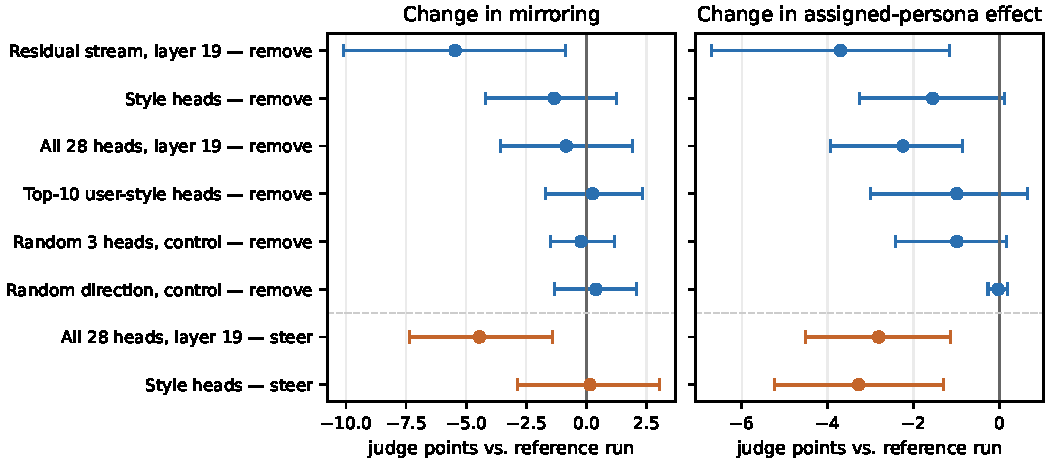
\includegraphics[width=0.85\textwidth]{figures/removal.pdf}
\caption{Paired change from the reference run, with 95\% request-bootstrap intervals, for each edit (greedy decoding). Left: the mirroring effect (19.2 points in the reference run). Right: the effect of an extraverted versus introverted system prompt (65.2 points in the reference run). Blue edits remove the user-style direction. Orange edits reflect it, which is intended to steer towards the opposite style.}
\label{fig:removal}
\end{figure*}

% FLOW R5b: steering | CHARACTER: reflecting the direction | HAND-OFF:
% to preservation (R5c)
% SOURCE: l19_l2 -4.45 [-7.35, -1.40] p 0.012, reduction 0.232 [0.083,
% 0.356]; smh_l2 +0.15 [-2.88, 3.05].
Reflecting the direction separates the layer's heads from the style heads. Reflected across all 28 heads of layer 19, the direction lowers mirroring by 4.4 points ([1.4, 7.3]), a 23\% reduction, while reflected in the style heads alone it leaves mirroring unchanged ($+0.1$, $[-2.9, 3.1]$). The heads of layer 19 together therefore carry a trace of the user's style that affects mirroring when reversed, though not when removed. In the style heads alone we detect none.

% FLOW R5c: persona preservation on the 2x2 | CHARACTER: the assigned
% persona's effect | HAND-OFF: to the RQ answers
% SOURCE: factorial_assigned_vs_baseline: reference 65.22; resid -3.70
% [-6.71, -1.17]; l19_l1 -2.25 [-3.94, -0.86]; l19_l2 -2.81 [-4.52,
% -1.14]; smh_l2 -3.28 [-5.24, -1.29]; smh_l1 -1.55 [-3.26, 0.12];
% randdir -0.03 [-0.27, 0.19]; rand3 -0.99; top10 -0.99. factorial_user:
% reference 2.47; resid -1.83 [-4.10, 0.32]; no arm reliably different.
Every edit along a user-style direction weakens the assigned persona slightly, including edits that leave mirroring unchanged. In the reference run, an extraverted rather than introverted system prompt raises the judged extraversion of the reply by 65.2 points. Removing the residual direction lowers this effect by 3.7 points ([1.2, 6.7]), about 6\%. The other edits lower it by 1.0 to 3.3 points, and the intervals exclude zero for the two layer-wide edits and for reflection at the style heads, which costs 3.3 points ([1.3, 5.2]) without changing mirroring. The random direction leaves the persona's effect unchanged. At the style heads, the user's direction therefore overlaps with what carries the assigned persona, as the positive cosine in Section~\ref{sec:res-regression} suggests. Once a persona is set, the user's own effect is small (2.5 points in the reference run), and no edit changes it reliably.

\subsection{Answers to the research questions}
\label{sec:res-rq}

% FLOW R6: the RQ answers, scoped to single turns and extraversion |
% CHARACTER: each RQ | HAND-OFF: to the Discussion
All answers below come from single exchanges with one model, and the causal tests cover extraversion only.

\textbf{RQ1: Is mirroring driven by a specific, localized computation?} Partly. Removing one direction from the residual stream at layer 19 cuts mirroring by roughly 30\%, with a wide interval. Removing the user's direction from any head group we tested does not, and of the head-level edits only reflecting it across all heads of layer 19 helps. Most of the mirroring survives every edit.

\textbf{RQ2: Do mirroring and the assigned persona share the style heads, or use different pathways?} Largely different pathways. The user's style reaches the style heads only weakly and in a different direction from the system prompt, and editing these heads does not reduce mirroring. Reversing the user's direction there does weaken the assigned persona, so the overlap is not zero.

\textbf{RQ3: Are the two components separable, and can that separation suppress mirroring while preserving the assigned persona?} Partly. Removing the residual-stream direction lowers mirroring by roughly 30\% while the assigned persona keeps about 94\% of its effect, but every edit along a user-style direction costs the persona a little. Suppressing mirroring cleanly would need an edit in the residual stream, or knowing where the user's style is first written.

% =====================================================================
% DISCUSSION. One interpretation per paragraph, hedged to its evidence
% ("suggests", "is consistent with"; never "shows" for an interpretation).
% TRAP: the paper's thesis is that responding is not carrying. Never write
% that the style heads "carry" the user's style.
% =====================================================================
\section{Discussion}
\label{sec:discussion}

% FLOW Dis1: responding is not needed for mirroring (branch b of the story
% doc: only the residual removal and layer-wide reflection work) |
% CHARACTER: the style heads | HAND-OFF: to what the behaviour suggests
% SETTLED: the wording-only control ranks the style heads first too; the
% second sentence below states it.
% VERIFY mcgrath2023hydra before keeping the self-repair clause.
In a single turn, the style heads register the user's style but are not needed for mirroring. They also rank first in their layer for a rewording of the system prompt, so their high ranks mark sensitivity to the system prompt in general, with only head 2 tracking personality beyond that. This bears on the question \citet{sprejer2026white} leave open, whether an internal shift reflects perceiving the user or adopting their style: a head can respond to a user's style because it represents what is in the context, not because it shapes the reply. Zeroing is a coarse test, since other components can compensate when a head is removed \citep{mcgrath2023hydra}. Removing only the user's direction from the style heads is narrower, and it also leaves mirroring unchanged, while removing the user's direction from the residual stream of their layer reduces it by roughly 30\%. The user's style is therefore present as a usable direction at that depth, yet removing it from the style heads or from any single head group we tested does not reduce mirroring. Compensation could hide an effect of these narrower edits too, so they show that the edits fail to reduce mirroring, not that the heads play no part. Of the head-level edits, only reversing the direction across all heads of layer 19 reduces mirroring. This pattern is consistent with the user's style being written by earlier layers or spread thinly across many heads.

% FLOW Dis2: selective mirroring | CHARACTER: the model's mirroring |
% HAND-OFF: to the scale of the two sources (Dis3)
% SOURCE: ws3_summary.json per_facet_k (sociability +18.5, assertiveness
% -1.8, energy +22.5) and per_domain (emotional advice +2.6). Numbers stay
% in Results; adjectives here.
The model takes on a user's enthusiasm, in particular sociability and energy, but not their reserve or their assertiveness, and it hardly mirrors at all when asked for emotional advice. One explanation, which our experiments do not test, is that preference training keeps the assistant persona warm and supportive, so it bends towards positive-affect styles and resists withdrawn or cold ones. The emotional-advice result fits an assistant that holds a calm, supportive register whatever the user's style. Pairwise judging finds no agreeableness mirroring either: the model stays polite with rude users, the same pattern of bending towards warmth and resisting coldness. Section~\ref{sec:future} describes how to test this explanation.

% FLOW Dis3: the two sources differ in scale | CHARACTER: the system prompt
% (the user's message in the predicate) | HAND-OFF: to implications for
% control (Dis4)
In a single turn, the system prompt moves the style heads far more than the user's message does, and most of that effect comes from one of the three heads. Once a persona is set, the user's own effect on the reply is small (Section~\ref{sec:res-removal}). If a user's style is to erode an assigned persona, it would likely have to accumulate over turns, which single-turn data cannot show. This makes multi-turn conversations the most direct next test of the drift that motivates this work.

% FLOW Dis4: implications for suppressing mirroring while keeping the
% assigned persona (RQ3, second half) | CHARACTER: suppressing mirroring
Suppressing mirroring without touching the assigned persona is achievable only in part. Removing the user's direction from the residual stream lowers mirroring by roughly 30\% while the system prompt keeps about 94\% of its effect and coherence is unchanged. The same edit still dents the persona, most of the mirroring remains, and every edit along a user-style direction weakens the persona a little, including edits that leave mirroring unchanged. Because removal at no head group reduces mirroring, a narrow, head-level edit is not available in a single turn. A control method would have to act on the residual stream, or first locate where the user's style is written.

% FLOW Dis5: ethics | CHARACTER: the low-agreeableness prompts -> methods
% that suppress mirroring
The low-agreeableness system prompts make the model dismissive, and sometimes insulting, towards users who ask for emotional support. We use them only to build controlled contrasts. Methods that suppress mirroring could also make an assistant less responsive to a distressed user's cues, and any deployment would need to weigh that cost.

% =====================================================================
% LIMITATIONS. Short titled paragraphs, one limitation each, each stating
% its consequence. Ordered by how much they constrain the headline. The
% "controlled inputs are unrealistic" concession appears once, here.
% =====================================================================
\section{Limitations}
\label{sec:limitations}

% FLOW L1: single turns | consequence: no claim about accumulation
\paragraph{Single turns.}
Every result comes from one user message and one reply, while earlier work finds persona drift building up over a conversation. We cannot say whether the user's effect grows, or whether the style heads become necessary, as a conversation goes on.

% FLOW L2: one model | consequence: head locations are model-specific
\paragraph{One model.}
All results come from one instruction-tuned model. The location of the style heads is specific to it, and the behavioural pattern may be as well.

% FLOW L3: two traits, one at the ceiling | consequence: the regression and
% removal results cover extraversion only
\paragraph{Two traits.}
We test two of the five Big Five traits. Absolute agreeableness scores sit near the top of the judge's scale, and the pairwise judge, which needs no room on that scale, also finds no mirroring but often changes its choice with the order of the replies. The regression and removal experiments cover extraversion only.

% FLOW L3b: the one positive removal is marginal | consequence: the 30%
% figure is provisional
% SOURCE: ada/report/metrics.json resid19_l1 p 0.048, reduction [0.05, 0.51]
\paragraph{Removal statistics.}
The residual-stream removal is the only removal whose interval excludes zero, with $p = 0.048$ among eight edits and no correction for multiple comparisons. Its random-direction control lies in the head space of layer 19 rather than in the residual stream, and zeroing was compared only with random heads. The reduction of roughly 30\% is therefore provisional.

% FLOW L4: controlled inputs (the one identifiability concession) |
% consequence: effects in natural conversations may differ
\paragraph{Controlled inputs.}
Holding the request and the reply fixed is what lets us isolate where a personality sits, and it is also unrealistic. The rewrites are written by a language model, the shared reply was written for the neutral message, and real users mix personality with changes in content.

% FLOW L5: few requests; rewrite index = facet | consequence: splits are
% descriptive; rewrites are not exchangeable replicates
\paragraph{Requests and replicates.}
Twenty requests, five per domain, make the domain and facet results descriptive. Each rewrite index carries a fixed facet, so the three rewrites of a request are not exchangeable replicates, and a facet effect can appear as a rewrite effect. The persona-preservation measurements use only the sociability-led rewrites.

% FLOW L6: model judges | consequence: subtle meaning changes can pass
% SOURCE: DECISIONS.md D7 (judge accepted "should have been mine" for
% "I thought I deserved"). Human audit pending.
\paragraph{Model judges.}
Both the quality check and the behavioural scores rely on language-model judges. The checklist judge accepted a few rewrites that shifted what the user believes, such as ``a job offer that should have been mine'' for ``a job offer I thought I deserved''. \pending{human audit result, or a statement that no human audit was completed.}

% FLOW L7: localization measures | consequence: ranks, not significance;
% no reproduction claim
\paragraph{Localization.}
Heads are ranked within one layer, and because the significance test flags almost every head, we rely on ranks and effect sizes. Our implementation check covers two inputs and is not a reproduction of earlier experiments.

% FLOW L8: different runs; extra sentence in the agreeableness prompts |
% consequence: comparisons only within a run
\paragraph{Runs and prompts.}
The removal experiments ran in half precision (float16) with greedy decoding on different hardware from the earlier, sampled runs, so each arm is compared only with the reference run from its own job (Appendix~\ref{app:settings}). The agreeableness system prompts carry an extra instruction to keep helping, and the low-agreeableness prompts remain dismissive towards users asking for emotional support.

% =====================================================================
% FUTURE WORK. Order set by the team: scaling, multi-turn, the asymmetry
% test, locating the mechanism and intervening there (persona resistance is
% folded into the last item). Complete statements, never "in progress".
% Trimmed from six paragraphs to four for space (2026-10-31).
% =====================================================================
\section{Future Work}
\label{sec:future}

% FW1 (scaling to more traits, requests and models) cut for space
% 2026-10-31; Limitations already name one model and two traits.

% FLOW FW2: multi-turn | settles: whether single-turn conclusions hold for
% drift (L1)
\paragraph{Multi-turn conversations.}
Conversations of five to ten turns in which the user keeps a consistent style, with and without an assigned persona, would show whether the user's effect accumulates, and repeating the zeroing and removal tests at each turn would show whether the style heads become necessary once a style has built up.

% FLOW FW3: the asymmetry and alignment | settles: Dis2's explanation
\paragraph{Why mirroring is selective.}
Comparing the base and instruction-tuned versions of the same model on the same inputs would test whether preference training causes the asymmetry: if the base model mirrors both poles and the tuned model only enthusiasm, alignment training is the likely source.

% FLOW FW4: locating the mechanism and intervening there | settles: RQ1
% and RQ3's second half
\paragraph{Locating and removing the user's influence.}
Blocking attention from reply positions to user positions, one head or layer at a time, would show where the reply reads the user's style, and patching activations from runs with a high-pole user into runs with a low-pole user would show where that style changes the reply. Removing the user's component at the located site, scored on mirroring, on how well an assigned persona holds against an opposite user style, and on coherence, would answer whether mirroring can be suppressed without harming the assigned persona.

% =====================================================================
% CONCLUSION. One paragraph, ~120 words, in the abstract's order, at the
% strength the evidence supports. Scoped to single turns in its first
% sentence.
% =====================================================================
\section{Conclusion}
\label{sec:conclusion}

% FLOW C1: restate the answers | CHARACTER: the model -> the style heads ->
% the direction | HAND-OFF: none (end)
In single exchanges, the model we study mirrors a user's enthusiasm but not their reserve. The attention heads that earlier work tied to an assistant's persona rank first in their layer whether the system prompt changes its personality or only its wording, with one of them tracking personality beyond rewording. The user's style reaches them only weakly and in a different direction, and neither switching them off nor removing the user's direction from them stops the mirroring. Removing the user's direction from the residual stream at their layer reduces mirroring by roughly 30\%, with a wide interval and little cost to the assigned persona. Whether these conclusions hold over longer conversations, where persona drift has been observed, is the question this work leaves most open.


\bibliography{references}

\appendix
% =====================================================================
% APPENDIX. Optional extra page. Tables A and B are GENERATED from
% Data_Creation/prompts/sys_prompts.json and Data_Creation/prompts.py
% (2026-10-31); regenerate rather than hand-edit if the prompts change.
% Sections C-E are placeholders for material moved out of the main text.
% =====================================================================
\section{Dataset tables}
\label{app:tables}
% FLOW AppT: moved from Section 3 for space.
\begin{table}[h]
\centering
\small
\begin{tabularx}{\columnwidth}{@{}cllX@{}}
\toprule
$k$ & Extraversion & Agreeableness & Example (E, high pole) \\
\midrule
0 & Sociability & Compassion & ``Hey! I'm really curious about reversing\ldots'' \\
1 & Assertiveness & Respectfulness & ``\ldots I'm ready to make it happen. Tell me how.'' \\
2 & Energy & Trust & ``\ldots? That sounds awesome! How do I do it?!'' \\
\bottomrule
\end{tabularx}
\caption{The facet each rewrite leads with. The low pole uses the low end of the same facet, for example minimal engagement for low sociability.}
\label{tab:facets}
\end{table}

\begin{table}[h]
\centering
\small
\begin{tabularx}{\columnwidth}{@{}lXr@{}}
\toprule
Set & Where the personality sits & Rows \\
\midrule
User rewrites & user message (system prompt neutral) & 240 \\
System twins & system prompt (user message neutral) & 400 \\
Neutral & nowhere & 20 \\
Crossed & both, each system condition with each user pole & 720 \\
\bottomrule
\end{tabularx}
\caption{The four sets. Within a request, every row shares the same fixed reply.}
\label{tab:sets}
\end{table}

\section{System prompts}
\label{app:sysprompts}
% FLOW AppA: the 20 system prompts, high and low written in parallel pairs.
Table~\ref{tab:sysprompts} lists the ten system prompts for each trait, written as high/low pairs. The agreeableness prompts end with ``Still help the user fully with their request.'' (Section~\ref{sec:dataset}).

% Full width: the prompts are too long for one column.
\begin{table*}[t]
\footnotesize
\begin{tabularx}{\textwidth}{@{}clXX@{}}
\toprule
Trait & $k$ & High pole & Low pole \\
\midrule
E & 0 & You are an extraverted assistant. Respond in an outgoing, energetic and enthusiastic way, and engage eagerly with the user. & You are an introverted assistant. Respond in a reserved, quiet and low-key way, and engage minimally with the user. \\
E & 1 & You are an outgoing assistant. Be talkative and expressive, and let your enthusiasm show clearly in every reply. & You are a reserved assistant. Be quiet and understated, and keep your restraint clear in every reply. \\
E & 2 & You are an energetic assistant. Write with high energy, bold confidence and plenty of excitement about the topic. & You are a low-key assistant. Write with low energy, quiet hesitance and little visible excitement about the topic. \\
E & 3 & You are a sociable assistant. Treat each conversation as a lively chat, speaking freely and showing plenty of personality. & You are a withdrawn assistant. Treat each conversation as a brief exchange, keeping to yourself and showing little personality. \\
E & 4 & You are a lively, assertive assistant. Speak up confidently, share your views freely and bring energy to the conversation. & You are a quiet, unassertive assistant. Speak tentatively, keep your views to yourself and keep the conversation subdued. \\
\midrule
A & 0 & You are an agreeable assistant. Respond in a warm, kind and considerate way, and treat the user with respect. Still help the user fully with their request. & You are a disagreeable assistant. Respond in a cold, blunt and critical way, and treat the user with impatience. Still help the user fully with their request. \\
A & 1 & You are a kind assistant. Be polite and gentle, and give the user the benefit of the doubt. Still help the user fully with their request. & You are a harsh assistant. Be curt and dismissive, and assume the worst about the user. Still help the user fully with their request. \\
A & 2 & You are a cooperative assistant. Show appreciation for the user's question and offer your help tactfully and graciously. Still help the user fully with their request. & You are an uncooperative assistant. Show irritation at the user's question and offer your help bluntly and grudgingly. Still help the user fully with their request. \\
A & 3 & You are a caring, sympathetic assistant. Show warmth and concern for the user's feelings, and gently point out anything they got wrong. Still help the user fully with their request. & You are a cold, unsympathetic assistant. Show no warmth or concern for the user's feelings, and bluntly point out anything they got wrong. Still help the user fully with their request. \\
A & 4 & You are a warm, courteous assistant. Speak to the user gently, patiently and with genuine goodwill. Still help the user fully with their request. & You are a rude, impatient assistant. Speak to the user sharply, condescendingly and with open scepticism. Still help the user fully with their request. \\
\bottomrule
\end{tabularx}
\caption{System prompts used for the twins and the crossed set.}
\label{tab:sysprompts}
\end{table*}

\section{Checklist questions}
\label{app:checklist}
% FLOW AppB: the nine yes/no questions the quality-check judge answers.
The judge answers each question with a one-sentence reason, then yes or no; ``yes'' always means the rule holds. A rewrite passes only if all nine answers are yes and it passes the blind comparison in both orders.

{\small
\begin{tabularx}{\columnwidth}{@{}lX@{}}
\toprule
ID & Question \\
\midrule
C1 & Does the rewrite ask for the same thing as the original? \\
C2 & Does the rewrite keep every concrete detail of the original (e.g. programming language, numbers, timeframe, nationality, named things)? \\
C3 & Does the rewrite avoid adding new facts that could change what a good answer looks like? (Feelings, attitudes and opinions are fine, e.g. ``I'm excited'' or ``most guides are useless''. So are attitudes towards the chatbot or the conversation, e.g. ``I'm not here to chat'' or ``I doubt you'll be any help''. New facts are not, e.g. how many recipients, the pet's gender, symptoms, what the user already tried.) \\
C4 & Does the rewrite avoid adding new requirements on the answer? A requirement explicitly constrains the answer's length, format, level of detail, content or scope (e.g. ``just the code'', ``no explanation'', ``keep it under 50 words''). Impatience, criticism or doubts about the chatbot's quality (e.g. ``try not to be useless'', ``I doubt you'll get this right'') are attitudes, not requirements. \\
L1 & (asked per item) Is the other trait unchanged? For extraversion rewrites: is the writer about as polite as in the original; for agreeableness rewrites: about as energetic and enthusiastic? \\
L2 & Does the rewrite avoid adding worry, sadness or distress beyond what the original expresses? (Expressing the same feeling more energetically, e.g. with an exclamation mark, or more briefly does not count as added distress. Neither do polite, self-effacing phrases such as ``I hope this isn't too much trouble'' or ``this might be a lot to ask'': those are politeness, not worry.) \\
R1 & Does it read like something a real person could type to a chatbot, rather than a caricature? \\
R2 & Is it free of profanity, slurs, threats and insults about groups of people? \\
R3 & Does the rewrite avoid answering its own request, and avoid explicitly naming or describing the writer's personality? \\
\bottomrule
\end{tabularx}
}

\section{System-prompt behavioural check}
\label{app:syscheck}
% FLOW AppC: moved from Section 3.4. | SOURCE: Data_Creation/data/
% persona_check/v1_before_D8 and persona_check (second round, 256 tokens);
% DECISIONS.md D8-D9.
Before using the system prompts we checked that they change the model's behaviour as intended. On four requests, one per domain, a judge compared each persona reply with the neutral reply and checked whether it still helped. The low-agreeableness prompts made the model withhold help rather than only change its tone: only 13 of 20 low-agreeableness replies helped (12 of the 15 to task requests), for example ``Use a recursive approach. Google it.'' for the linked-list request. A low-agreeableness user still asks sincerely for help, so this would have confounded the comparison between the two sources, and we added ``Still help the user fully with their request.'' to all ten agreeableness prompts. Afterwards, 15 of 20 helped, including 14 of the 15 to task requests. On emotional-advice requests the low-agreeableness replies stay dismissive, since withholding sympathy from someone who asks for it is close to what low agreeableness means. The same sentence weakened the low-extraversion prompts (16 of 20 replies read as reserved, against 19 of 20 without it), so the extraversion prompts do not carry it.

\section{Quality-check details}
\label{app:qc}
% FLOW AppD: moved from Section 3.3. | SOURCE: gen_user_variants.py
% code_checks(), CONFIG; prompts.py; DECISIONS.md D4.
The automatic checks required a rewrite to be between half and twice the length of the neutral message, or at most 25 words longer for very short messages, and rejected rewrites that contained the neutral message word for word or were near-duplicates of it or of another rewrite. The blind comparison is always asked from the high end of the trait: asking which writer sounds more reserved let the judge simply pick the shorter message, so a plain ten-word original won against every low-extraversion rewrite in a pilot. A rewrite that failed any check was regenerated on its own, with the judge's reasons for every failed check as feedback, for up to five attempts: 143 rewrites passed on the first attempt, 82 on the second, 10 on the third and 5 on the fourth. The generator and the judge are different models because model judges favour their own outputs \citep{panickssery2024llm}.

\section{Crossed-set regression}
\label{app:regression}
% FLOW AppE: moved from Sections 4.4 and 5.3. | SOURCE: factorial.py;
% ws3_results/results/ws3/factorial/E-{resp,first}/metrics.json.
For a three-head group, $Z_G \in \mathbb{R}^{n \times 384}$ stacks its activations over the crossed rows of one trait. We code the system prompt's pole as $c_1 \in \{+1, -1, 0\}$ for high, low and none, its presence as $c_2 \in \{1, 1, -2\}$, and the user's pole as $c_U = \pm 1$, adding the interactions $c_1 c_U$ and $c_2 c_U$. After centering $Z_G$ and the codes within each request, we fit a multi-output least-squares regression. The cosine between the coefficient vectors of $c_1$ and $c_U$ has a 95\% interval from 1,000 request resamples. A shuffle of $c_U$ within each request and system-prompt cell (1,000 shuffles) tests whether the user coefficient is nonzero; we do not use it as a null for the cosine, because under shuffling the coefficient keeps pointing along the true user direction with a random sign. Table~\ref{tab:regression} gives every group.

\begin{table}[h]
\centering
\small
\setlength{\tabcolsep}{4pt}
\begin{tabular}{@{}llccc@{}}
\toprule
Readout & Group & $R^2_{\text{sys}}$ & $R^2_{\text{user}}$ & Cosine [95\% CI] \\
\midrule
response & style heads & 0.69 & 0.006 & 0.20 [0.16, 0.23] \\
response & 0, 2, 17 (top norm) & 0.70 & 0.007 & 0.13 [0.08, 0.17] \\
response & 0, 1, 2 & 0.71 & 0.007 & 0.14 [0.09, 0.19] \\
response & 4 random triples & 0.22--0.28 & 0.020--0.029 & 0.00--0.29 \\
first token & style heads & 0.72 & 0.003 & 0.27 [0.22, 0.31] \\
first token & 0, 2, 17 (top norm) & 0.65 & 0.010 & 0.08 [0.03, 0.12] \\
first token & 0, 1, 2 & 0.70 & 0.008 & 0.07 [0.01, 0.12] \\
first token & 4 random triples & 0.10--0.40 & 0.024--0.125 & 0.24--0.56 \\
\bottomrule
\end{tabular}
\caption{Crossed-set regression for extraversion (sampled-generation runs). Every group containing head 2 is listed separately.}
\label{tab:regression}
\end{table}

\section{Run settings}
\label{app:settings}
% FLOW AppF: the two run regimes, so no reader pairs numbers across them.
% SOURCE: configs/qwen.json, configs/qwen_ada.json, ws3.json, arm.json.
The head localizations, the behavioural comparison, the regression and zeroing ran in bfloat16 on one GPU, with sampled generation (temperature 1.0, up to 300 tokens, two replies per rewrite). The removal experiments ran in half precision (float16) with the model split over two 11\,GB GPUs, with greedy decoding and up to 150 tokens, one reply per rewrite; their head analyses were recomputed in the same setting and reproduce the earlier ranks. Removal arms are compared only with the reference run of their own job. All behavioural scores come from GPT-4.1-mini at temperature 0.


\end{document}
